% =============================================================================
% Working extract -- full dissertation appendix (Data, Methodology, and Results,
% all three Qs). Renamed from appendix_results.tex 2026-08-23 and scope widened --
% the old Results-only restriction below no longer applies, since Data/Methodology
% appendix material is now being built up here too, not deferred.
% Content fragment, NOT a standalone compilable document -- meant to be merged
% into the main file's existing \chapter{Appendix} \label{chap:appendix} in
% 20th_1_31_pm_audited.tex (currently an empty placeholder chapter, see its own
% % AUDIT: note listing 7 unresolved \ref calls).
%
% Structure: \chapter{Data}, \chapter{Methodology}, then one \section per research
% question for Results-appendix material (matching the three working results_qN_*.tex
% files). Built content is filled in as it's ready; not-yet-built content is a short
% placeholder note, not invented numbers.
% =============================================================================

\chapter{Data}

\section{Field derivations and forestry definitions}
\begin{table}[!htbp]
\centering
\scriptsize
\setlength{\tabcolsep}{3pt}
\renewcommand{\arraystretch}{1.05}
\begin{tabular}{p{2.1cm}p{4.6cm}p{4.6cm}p{3.4cm}}
\hline
Term & Formula & Forestry meaning (with units) & Used in this project \\
\hline
\texttt{Age} & $\texttt{LiDAR\_year} - \texttt{plyr}$ & Stand age at the survey date, in years since planting & Modelling input; cleaning filter. \fc{Field-description doc states valid range 0--150 years; \texttt{clean\_master\_data.py} implements 0--200 -- documentation/code mismatch, unresolved} \\
\texttt{Top\_Height95} & $\texttt{elev\_percentile\_95th}\times1.1$ & FR's corrected estimate of Top Height (m): mean height of the 100 largest-diameter trees per hectare. The $\times1.1$ factor is FR's stated correction for known underestimation at the 95th return percentile & Audit ingredient only (feeds
\texttt{Vol95}/\texttt{GYCspec95}). This project's target is the \emph{uncorrected} \texttt{elev\_percentile\_95th} -- a deliberate deviation from FR's own corrected convention \\
\texttt{Vol95} & $(g_1\cdot\texttt{Top\_Height95}^{g_3})\times(\texttt{area}/10000)\times\texttt{CanopyCover}$ & Stand volume (m\textsuperscript{3}), scaled from a per-ha allometric relationship by plot area (ha) and canopy cover fraction & Used downstream as a disturbance-screening signal. $g_1$/$g_3$ are pre-assigned per plot in the source FR export, not computed or selected by this project -- e.g.\ $g_1{=}3.509144,\,g_3{=}1.478136$ and $g_1{=}2.922183,\,g_3{=}1.694732$ are two real examples. % Verified 2026-08-23 against clean_master_4survey.parquet: SS alone has 10 distinct (g1,g3) pairs, not split cleanly by thinning status (6 of the 10 pairs occur under BOTH Thin=0 and Thin=1) or by yield class (each pair spans 7-12 different yldc values) -- the true determinant isn't visible in this project's own tables, likely region or an internal FR yield-model version. Do not describe this as "N pairs per thinning status" or imply thinning/yldc determines the pair.
\\
\texttt{Vol\_RM95} & $(-35.8733+5.3486\cdot\texttt{Top\_Height95}^{1.5424})\times(\texttt{area}/10000)\times\texttt{CanopyCover}$ & Robertson \& Miller generic volume equation (m\textsuperscript{3}), species-independent alternative to \texttt{Vol95} & Not kept in the master export; not used \\
\texttt{GYCspec95} & $\bigl(\texttt{Top\_Height95}/(1-e^{-p_4\cdot\texttt{Age}})^{p_5}-p_1-p_3\times2\bigr)/p_2$ & General Yield Class (continuous scale; FR's own tables report GYC in multiples of 2, e.g.\ YC14, YC16): potential productivity, the maximum mean annual increment of cumulative volume
(m\textsuperscript{3}/ha/yr) for the species on that site under standard management & Never used downstream; would be leakage if it were (contains \texttt{Top\_Height95}) \\
$y_{\max}^{\texttt{yldc}}$ (RQ3) & $\texttt{yldc}\cdot p_2+p_1+p_3\times2$ & The height ceiling (m) that the plot's independently assigned yield class implies, under the same site-index model as \texttt{GYCspec95}, solved the opposite direction & Used -- RQ3's independent comparison baseline
(\texttt{data\_processing/export\_growth\_curve\_tables.py}) \\
\texttt{DBHmean} \ct{source PDF/report, not yet in citation list} & $(b_1+b_2\cdot\texttt{Spacing})\times\texttt{TopHeight}^{b_4}$ & Mean diameter at breast height, 1.3\,m above ground (cm); needed to estimate stems per hectare & \textbf{Not present anywhere in this project's data or code.} Supporting context only, for the
claim that top height feeds an established forestry allometric toolkit (SS, thinned: $b_1{=}0.714157,\,b_2{=}0.239399,\,b_4{=}1.079545$; unthinned: $b_1{=}1.212457,\,b_2{=}0.609335,\,b_4{=}0.754978$) \\
\texttt{BA} \ct{same source} & $h_1\times\texttt{TopHeight}^{h_4}$ & Basal area (m\textsuperscript{2}/ha): cross-sectional stem area summed per hectare & Not present in this project's data. Same supporting-context caveat (SS, thinned: $h_1{=}7.499437,\,h_4{=}0.497925$; unthinned: $h_1{=}5.517392,\,h_4{=}0.771801$) \\
Volume (source PDF, Eq.~13) \ct{same source} & $g_1\times\texttt{TopHeight}^{g_3}$ (no area/canopy scaling) & Volume over bark, per hectare (m\textsuperscript{3}/ha) & \fc{Distinct equation from this project's own \texttt{Vol95} above -- same $g_1$/$g_3$ notation, different formula (no area/\texttt{CanopyCover} scaling). Do
not conflate the two in the appendix text} \\
Top Height (forestry definition) & -- & Mean height of the 100 largest-diameter trees per hectare (m) & \texttt{elev\_percentile\_95th} is an ALS-derived proxy for this classical mensuration concept, not identical to it by construction \\
Yield Class (forestry definition) & -- & Index of site productivity: max mean annual increment of cumulative volume (m\textsuperscript{3}/ha/yr); tabulated in multiples of 2 in FR yield tables, continuous here & \texttt{yldc} is this project's realisation of it \\
\hline
\end{tabular}
\caption{Full derivation and forestry definitions for fields referenced in Table~\ref{tab:data-fields} but not spelled out there. Units given wherever the source defines them.}
\label{tab:appendix-formulas}
\end{table}

\section{Environmental variable definitions and coverage}
% Filed under Data, not Methodology, despite the source draft's "METHODLOGOY" heading --
% this table's own caption says feature-selection/VIF/final model membership are described
% in the Methodology chapter, "not here". What's actually here (extraction method, coverage,
% distinct values, min/max per raw variable) is Data-chapter material -- variable definitions,
% not model construction. Moved 2026-08-23; flag if this placement is wrong.
\begin{table}[!htbp]
\centering
\tiny
\setlength{\tabcolsep}{2pt}
\renewcommand{\arraystretch}{0.9}
\begin{tabular}{p{2.3cm}p{1.6cm}p{3.0cm}p{1.3cm}p{1.1cm}p{2.3cm}}
\hline
Variable & Family & Extraction method & Valid/ Missing & Distinct & Min--Max \\
\hline
\texttt{elevation} & Terrain & Direct raster read & 71{,}766/0 & 4{,}028 & 18.2--561.1\,m \\
\texttt{slope\_degrees} & Terrain & $\arctan(\sqrt{dz_{dx}^2+dz_{dy}^2})$, \texttt{np.gradient} & 71{,}766/0 & 15{,}326 & 0.0--42.84$^\circ$ \\
\texttt{northness}, \texttt{eastness} & Terrain & $\cos/\sin$(aspect, radians) & 71{,}766/0 & 15{,}387/15{,}572 & $-1$--$1$ \\
\texttt{profile\_/plan\_curvature} & Terrain & 2nd derivative of DTM \citep{zevenbergen1987} & 71{,}766/0 & 16{,}835/16{,}829 & $-0.007$--$0.008$ / $-0.67$--$0.40$ \\
\texttt{local\_relief\_500m} & Terrain & Max$-$min elevation, 21$\times$21-cell window & 71{,}766/0 & 6{,}086 & 7.5--461.9\,m \\
\texttt{solar\_radiation\_index} & Terrain & $\cos(\text{slope})\cos(\text{zenith})+\sin(\text{slope})\sin(\text{zenith})\cos(\text{aspect}-\text{azimuth})$, no horizon shading & 71{,}766/0 & 16{,}012 & 0.338--1.000 \\
\texttt{frost\_hollow\_flag} & Terrain & Binary: TPI $<$ own 15th pctile AND plan curvature $<0$ & 71{,}766/0 & 2 & 0 ($n{=}62{,}691$)/1 ($n{=}9{,}075$) \\
\texttt{ceh\_twi} & Terrain & Direct raster read (CEH TWI) & 71{,}727/39 & 16{,}800 & 3.75--16.86 \\
\texttt{topex} & Wind & Sum of horizon angles, 8 directions \citep{wilson1984} & 71{,}766/0 & 16{,}839 & $-85.9$--$68.6^\circ$ \\
\texttt{windward\_topex} & Wind & Same, single 225$^\circ$ bearing & 71{,}766/0 & 8{,}093 & $-19.8$--$19.4^\circ$ \\
\texttt{gwa\_weibull\_a/k\_10m/50m} & Wind & Direct raster read, national grid & 71{,}766/0 & 1{,}816--1{,}824 & varies by variable \\
\texttt{gwa\_wind\_speed\_10m} & Wind & Nearest-cell extraction, REST API & 71{,}766/0 & 1{,}816 & 0.069--11.18\,m/s \\
\texttt{whcl} & Wind & Direct field read (raw GPKG) & 71{,}766/0 & 6 of 7 possible & Class 1 absent \\
\texttt{soilgrids\_ph} & Soil & Direct read, topsoil 0--5\,cm & 71{,}353/413 & 13 & 4.0--5.2 \\
\texttt{ceh\_pedotope} & Soil & Categorical, one-hot & 71{,}727/39 & 7 levels & -- \\
\texttt{ceh\_subsurface\_drainage} & Soil & Categorical, one-hot & 71{,}727/39 & 3 levels & -- \\
\texttt{ceh\_textural\_composition} & Soil & Categorical, one-hot & 71{,}727/39 & 4 levels & -- \\
\texttt{dist\_to\_watercourse} & Soil/spatial & Distance to nearest OS Open Rivers line & 71{,}766/0 & 71{,}758 & 0.0045--1850.9\,m \\
\texttt{chelsa\_gdd5\_degc} & Climate & Direct read, 1981--2010 & 71{,}766/0 & 206 & 906.5--1580.8 \\
\texttt{chelsa\_bio12\_precip\_mm} & Climate & Direct read, 1981--2010 & 71{,}766/0 & 269 & 1729.8--3004.8 \\
\texttt{tas\_mean}, \texttt{groundfrost\_mean} & Climate & Cohort-suffixed, resolved to cohort's real years & 71{,}766/0 & 149 each & 5.75--9.15 / 8.76--9.47 \\
\texttt{dist\_to\_scpt\_/\_block\_boundary} & Spatial & Distance to own sub-cpmt/block polygon & 71{,}766/0 & 68{,}188/53{,}974 & $\sim$0--217\,m \\
\texttt{dist\_to\_forest\_perimeter} & Spatial & Distance to buffered union of compartments & 71{,}766/0 & 71{,}701 & $\sim$0--764.7\,m \\
\texttt{cpmt\_compactness\_ratio} & Spatial & Perimeter/area, per compartment & 71{,}766/0 & 296 & 0.0097--0.240 \\
\texttt{dist\_to\_road} & Spatial & Distance to nearest OS Open Roads line & 71{,}766/0 & 71{,}580 & 0.056--2375.7\,m \\
\texttt{CanopyCover} & Stand & Mean fraction across survey years & 71{,}766/0 & 70{,}769 & 0.008--0.996 \\
\texttt{time\_since\_thinning} & Stand & NaN-filled with 0 downstream & 71{,}766/0 & 19 & 0--16\,yr \\
\hline
\end{tabular}
\caption{Per-variable definitions, extraction method and coverage for the environmental table
(71,766 plots). Source: \texttt{methodlogy\_env\_setpick.md}, verified 2026-08-10 against
\texttt{plot\_environmental\_features.parquet}. Feature-selection, VIF screening and which
variables entered a final model set are described in Chapter~\ref{ch:methodology}, not here.}
\label{tab:data-env-variables_detail_app}
\end{table}


\chapter{Methodology}

\section{Feature-set membership by research question}
\label{app:feature-sets}
% Converted from raw notes 2026-08-23. RSQ->Q mapping verified against actual production
% code (not just target-name matching): RSQ1 loads via models/common/torch_data.py's
% ENV_TERRAIN_FEATURE_SETS, which feeds Q3's DNN/PINN models directly (target
% elev_percentile_95th, confirmed both by that file's own TARGET_COLUMN and by
% feature_set_builder.py's own docstring: "RSQ1: ...feeds dnn_env_terrain/pinn_env_terrain*").
% RSQ2 loads in run_rq2_attribution.py, Q1's real production script (target
% mean_cr_residual). RSQ3 loads in run_rq3_gnnwr.py, Q2's real GNNWR production script
% (target local_y_max_difference). No mismatches found across every script checked.
%
% Machine-readable source: documentation/env_feature_sets_manifest.csv (225 rows) -- the
% snapshot below is for readability; the CSV is the definitive record if the two disagree.

Ranking and screening is repeated separately for each question's own target, so final Set
membership differs even where two questions share a Set number. Sets are not strictly nested:
VIF-based collinearity screening (variables with variance inflation factor $>5$ removed
iteratively) is re-run each time the candidate pool expands, so a variable present in a smaller
Set can be screened out once a larger Set's wider pool makes it redundant. Elevation is the
clearest example: it survives Set2 and Set3 in every question below, but is removed from Set4
once the wider terrain/wind pool is considered together -- this reflects statistical redundancy
with other terrain/wind variables (elevation is a well-known confound for temperature, wind
exposure and radiation), not that elevation is ecologically unimportant.

\subsection{Q1 (target \texttt{mean\_cr\_residual})}
\begin{table}[!htbp]
\centering
\scriptsize
\renewcommand{\arraystretch}{1.1}
\begin{tabularx}{\linewidth}{@{} l r >{\raggedright\arraybackslash}X @{}}
\toprule
Set & $n$ & Columns \\
\midrule
Set1 & 4 & \texttt{CanopyCover}, \texttt{time\_since\_thinning}, \texttt{time\_since\_thinning\_missing}, \texttt{recent\_thinning\_5yr} \\
Set2 & 14 & Set1 + \texttt{chelsa\_bio12\_precip\_mm}, \texttt{chelsa\_gdd5\_degc}, \texttt{gwa\_weibull\_k\_50m}, \texttt{slope\_degrees}, \texttt{gwa\_weibull\_a\_10m}, \texttt{local\_relief\_500m}, \texttt{eastness}, \texttt{dist\_to\_road}, \texttt{gwa\_weibull\_a\_50m}, \texttt{tas\_mean} \\
Set3 & 14 & Set1 + \texttt{gwa\_weibull\_k\_50m}, \texttt{slope\_degrees}, \texttt{gwa\_weibull\_a\_10m}, \texttt{local\_relief\_500m}, \texttt{eastness}, \texttt{gwa\_weibull\_a\_50m}, \texttt{ceh\_twi}, \texttt{whcl}, \texttt{topex}, \texttt{gwa\_wind\_speed\_10m} \\
Set4 & 19 & Set3 + \texttt{chelsa\_bio12\_precip\_mm}, \texttt{dist\_to\_road}, \texttt{tas\_mean}, \texttt{dist\_to\_scpt\_boundary}, \texttt{soilgrids\_ph} \\
Set5 & 28 & Set1 + \texttt{slope\_degrees}, \texttt{northness}, \texttt{eastness}, \texttt{profile\_curvature}, \texttt{plan\_curvature}, \texttt{tpi\_500m}, \texttt{local\_relief\_500m}, \texttt{frost\_hollow\_flag}, \texttt{windward\_topex}, \texttt{gwa\_weibull\_a\_10m}, \texttt{gwa\_weibull\_k\_10m}, \texttt{gwa\_weibull\_a\_50m}, \texttt{gwa\_weibull\_k\_50m}, \texttt{dist\_to\_forest\_perimeter}, \texttt{dist\_to\_block\_boundary}, \texttt{cpmt\_compactness\_ratio}, \texttt{dist\_to\_road}, \texttt{dist\_to\_watercourse}, \texttt{gwa\_wind\_speed\_10m}, \texttt{soilgrids\_ph}, \texttt{ceh\_twi}, \texttt{tas\_mean}, \texttt{groundfrost\_mean}, \texttt{whcl} \\
\bottomrule
\end{tabularx}
\caption{\small{Q1 (RSQ2) feature-set membership, elastic\_net/XGBoost/LMM attribution pipeline.}}
\label{tab:feature-sets-q1}
\end{table}

\subsection{Q2 (target \texttt{local\_y\_max\_difference})}
% ceh_* columns are one-hot dummy levels, reference level already dropped.
\begin{table}[!htbp]
\centering
\scriptsize
\renewcommand{\arraystretch}{1.1}
\begin{tabularx}{\linewidth}{@{} l r >{\raggedright\arraybackslash}X @{}}
\toprule
Set & $n$ & Columns \\
\midrule
Set1 & 4 & \texttt{CanopyCover}, \texttt{time\_since\_thinning}, \texttt{time\_since\_thinning\_missing}, \texttt{recent\_thinning\_5yr} \\
Set2 & 14 & Set1 + \texttt{windward\_topex}, \texttt{elevation}, \texttt{cpmt\_compactness\_ratio}, \texttt{gwa\_wind\_speed\_50m}, \texttt{slope\_degrees}, \texttt{tpi\_500m}, \texttt{dist\_to\_road}, \texttt{topex}, \texttt{solar\_radiation\_index}, \texttt{soilgrids\_ph} \\
Set3 & 12 & Set1 + \texttt{windward\_topex}, \texttt{elevation}, \texttt{gwa\_wind\_speed\_50m}, \texttt{slope\_degrees}, \texttt{tpi\_500m}, \texttt{topex}, \texttt{solar\_radiation\_index}, \texttt{northness} \\
Set4 & 20 & Set1 + \texttt{windward\_topex}, \texttt{gwa\_wind\_speed\_50m}, \texttt{slope\_degrees}, \texttt{tpi\_500m}, \texttt{topex}, \texttt{northness}, \texttt{cpmt\_compactness\_ratio}, \texttt{dist\_to\_road}, \texttt{chelsa\_bio12\_precip\_mm}, \texttt{tas\_mean}, \texttt{soilgrids\_ph}, \texttt{ceh\_subsurface\_drainage=2.0}, \texttt{ceh\_pedotope=2.0}, \texttt{ceh\_pedotope=8.0}, \texttt{ceh\_textural\_composition=2.0}, \texttt{dist\_to\_forest\_perimeter} \\
Set5 & 31 & Set1 + \texttt{slope\_degrees}, \texttt{northness}, \texttt{eastness}, \texttt{profile\_curvature}, \texttt{plan\_curvature}, \texttt{ceh\_twi}, \texttt{frost\_hollow\_flag}, \texttt{windward\_topex}, \texttt{whcl}, \texttt{tpi\_500m}, \texttt{local\_relief\_500m}, \texttt{tas\_mean}, \texttt{groundfrost\_mean}, \texttt{soilgrids\_ph}, \texttt{dist\_to\_watercourse}, \texttt{dist\_to\_forest\_perimeter}, \texttt{dist\_to\_scpt\_boundary}, \texttt{cpmt\_compactness\_ratio}, \texttt{dist\_to\_road}, \texttt{ceh\_pedotope=11.0}, \texttt{ceh\_pedotope=2.0}, \texttt{ceh\_pedotope=5.0}, \texttt{ceh\_pedotope=8.0}, \texttt{ceh\_pedotope=9.0}, \texttt{ceh\_subsurface\_drainage=2.0}, \texttt{ceh\_subsurface\_drainage=3.0}, \texttt{ceh\_textural\_composition=5.0} \\
\bottomrule
\end{tabularx}
\caption{\small{Q2 (RSQ3) feature-set membership, GNNWR spatial-attribution pipeline. Note Set3's non-monotonic size (12 columns, smaller than Set2's 14) is expected, not an error: Set2 and Set3 are built by two different rules (top-10 by rank vs.\ top-half-of-category by rank) over overlapping but not identical candidate pools -- Set3 is not defined as a superset of Set2.}}
\label{tab:feature-sets-q2}
\end{table}

\subsection{Q3 (target \texttt{elev\_percentile\_95th})}
\begin{table}[!htbp]
\centering
\scriptsize
\renewcommand{\arraystretch}{1.1}
\begin{tabularx}{\linewidth}{@{} l r >{\raggedright\arraybackslash}X @{}}
\toprule
Set & $n$ & Columns \\
\midrule
Set1 & 4 & \texttt{CanopyCover}, \texttt{time\_since\_thinning}, \texttt{time\_since\_thinning\_missing}, \texttt{recent\_thinning\_5yr} \\
Set2 & 14 & Set1 + \texttt{gwa\_weibull\_k\_50m}, \texttt{dist\_to\_scpt\_boundary}, \texttt{elevation}, \texttt{tas\_mean}, \texttt{eastness}, \texttt{windward\_topex}, \texttt{gwa\_weibull\_a\_10m}, \texttt{gwa\_weibull\_a\_50m}, \texttt{slope\_degrees}, \texttt{cpmt\_compactness\_ratio} \\
Set3 & 15 & Set1 + \texttt{gwa\_weibull\_k\_50m}, \texttt{elevation}, \texttt{eastness}, \texttt{windward\_topex}, \texttt{gwa\_weibull\_a\_10m}, \texttt{gwa\_weibull\_a\_50m}, \texttt{slope\_degrees}, \texttt{gwa\_weibull\_k\_10m}, \texttt{solar\_radiation\_index}, \texttt{ceh\_twi}, \texttt{gwa\_wind\_speed\_10m} \\
Set4 & 18 & Set1 + \texttt{gwa\_weibull\_k\_50m}, \texttt{eastness}, \texttt{windward\_topex}, \texttt{gwa\_weibull\_a\_10m}, \texttt{gwa\_weibull\_a\_50m}, \texttt{slope\_degrees}, \texttt{gwa\_weibull\_k\_10m}, \texttt{solar\_radiation\_index}, \texttt{ceh\_twi}, \texttt{gwa\_wind\_speed\_10m}, \texttt{dist\_to\_scpt\_boundary}, \texttt{tas\_mean}, \texttt{chelsa\_gdd5\_degc}, \texttt{cpmt\_compactness\_ratio} \\
Set5 & 30 & Set1 + \texttt{slope\_degrees}, \texttt{northness}, \texttt{eastness}, \texttt{profile\_curvature}, \texttt{plan\_curvature}, \texttt{local\_relief\_500m}, \texttt{frost\_hollow\_flag}, \texttt{topex}, \texttt{windward\_topex}, \texttt{gwa\_weibull\_a\_10m}, \texttt{gwa\_weibull\_k\_10m}, \texttt{gwa\_weibull\_a\_50m}, \texttt{gwa\_weibull\_k\_50m}, \texttt{dist\_to\_forest\_perimeter}, \texttt{dist\_to\_scpt\_boundary}, \texttt{cpmt\_compactness\_ratio}, \texttt{dist\_to\_road}, \texttt{dist\_to\_watercourse}, \texttt{gwa\_wind\_speed\_10m}, \texttt{soilgrids\_ph}, \texttt{ceh\_twi}, \texttt{chelsa\_gdd5\_degc}, \texttt{chelsa\_bio12\_precip\_mm}, \texttt{tas\_mean}, \texttt{groundfrost\_mean}, \texttt{whcl} \\
\bottomrule
\end{tabularx}
\caption{\small{Q3 (RSQ1) feature-set membership, DNN/PINN/PINN-$k$ prediction pipeline.}}
\label{tab:feature-sets-q3}
\end{table}

\subsection{Feature-set purpose by question}
% Renamed RSQ1->Q3, RSQ2->Q1, RSQ3->Q2 per the verified mapping above. "NLME" kept as the
% row label here since that's the actual module/function name in code (models/spatial_
% attribution/nlme.py) -- the main Methodology chapter calls the same model "linear mixed-
% effects model (LMM)" in prose; both names refer to the identical model, not two different
% ones. SCOPE_GROUPS claim ("no Q1 equivalent") verified by grep: SCOPE_GROUPS only appears
% in models/growth_curve_attribution/*.py (Q2's own module), nothing in models/spatial_
% attribution/ (Q1's module) -- but Q1 DOES have its own separate category-level ablation
% (the "soil +0.022, climate -0.056" result already in Results), just via a different,
% independent method, not this shared system. Both facts are true at once, not a contradiction.
\begin{table}[!htbp]
\centering
\scriptsize
\begin{tabularx}{\linewidth}{@{} l >{\raggedright\arraybackslash}X r r >{\raggedright\arraybackslash}X @{}}
\toprule
Feature set & Included feature groups & Model comparison & Environmental attribution & Reason \\
\midrule
Q3 (RSQ1) Set1--Set5 & Baseline + terrain/wind/climate/soil/edge (VIF-screened) & Yes (primary) & No & Feeds \texttt{dnn\_env\_terrain}/\texttt{pinn\_env\_terrain*} -- designed for a fair DNN-vs-PINN comparison under progressively richer environmental input, and to test whether environmental conditioning improves height prediction. No linear/coefficient model reads these; not designed for attribution. \\
Q1 (RSQ2) Set1--Set5 & Baseline + terrain/wind/climate/soil/edge (VIF-screened) & Secondary (Elastic Net vs.\ XGBoost vs.\ LMM/NLME) & Yes (primary) & Feeds Elastic Net/XGBoost/LMM on \texttt{mean\_cr\_residual} -- designed to identify which conditions align with persistent departure from the shared CR curve. Model comparison across the three fitted models is possible but secondary to the attribution question. \\
Q2 (RSQ3) Set1--Set5 & Baseline + terrain\_wind/climate/soil\_site/edge\_position (VIF-screened, one-hot, reference level dropped) & Secondary (Elastic Net vs.\ XGBoost vs.\ GNNWR) & Yes (primary) & Feeds Elastic Net/XGBoost/GNNWR on \texttt{local\_y\_max\_difference} -- per-plot attribution; GNNWR specifically tests whether attribution is spatially varying, not just globally linear. \\
Q2 (RSQ3) \texttt{SCOPE\_GROUPS} (pre-existing, untouched) & Named category combinations (\texttt{terrain\_wind}, \texttt{+climate}, \texttt{+soil\_site}, \texttt{+edge\_position}, \texttt{+management}, \texttt{broad\_environment}, \texttt{broad\_environment\_plus\_management}) & No & Yes (category-level) & A \emph{different}, coarser question -- "does adding this whole category help" -- answered by a pre-existing system this work did not modify. No Q1 equivalent of this specific system exists, though Q1 answers the same coarser question via its own separate category-ablation method (see Q1 appendix). \\
6-survey informational check (Q1/RSQ2 Set2 only) & Same candidate pool, 6-survey cohort & No & Diagnostic only & Not a primary result -- checks whether Set2's top-10 changes on the smaller (7,467-row), noisier 6-survey cohort. It does (only 1 of 10 candidates overlap with 4-survey's Set2) -- reported as a caveat on Set2's stability, not as a second deliverable. \\
\bottomrule
\end{tabularx}
\caption{\small{What each feature set is for, and which question(s) it serves. Widening a Set (Set2$\to$Set3$\to$Set4$\to$Set5) is not claimed to necessarily improve prediction or strengthen an attribution finding -- each Set is a candidate for downstream evaluation, and which one performs best is an empirical question for the project's real five-fold spatial CV, not decided by this screening pipeline.}}
\label{tab:feature-set-purpose}
\end{table}


\section{Q1 appendix}
\label{app:results-q1}

\subsection{Full Set4 variable table (EN vs.\ LMM, static/dynamic, stability)}
\label{app:nonlinearity-check}
% Referenced 3x from results_q1_21_08_0754pm.tex (the "one mechanism" paragraphs).
% Source: outputs/spatial_block_kfold/rq2_attribution_nested_set4_gated_all_vif/4survey/fold_{0-4}/,
% built 2026-08-21 -- see that file's own header comment for full provenance.

\begin{table}[!htbp]
\centering
\scriptsize
\setlength{\tabcolsep}{3pt}
\renewcommand{\arraystretch}{1.05}
\begin{tabular}{lrrllll}
\toprule
Variable & EN coef.\ (mean$\pm$SD) & LMM coef.\ (mean$\pm$SD) & Same sign? & Static/Dynamic & Stability verdict & Basis \\
\midrule
CanopyCover & $+1.943\pm0.038$ & $+1.864\pm0.078$ & Yes & Dynamic & Not assessed (leakage check instead) & -- \\
time\_since\_thinning & $-2.139\pm0.216$ & $-1.475\pm0.596$ & Yes & Dynamic & Not assessed & -- \\
time\_since\_thinning\_missing & $-2.995\pm0.182$ & $-1.321\pm0.698$ & Yes & Dynamic & Not assessed & -- \\
recent\_thinning\_5yr & $-0.975\pm0.273$ & $-0.403\pm0.286$ & Yes & Dynamic & Not assessed & -- \\
slope\_degrees & $+0.993\pm0.217$ & $+0.861\pm0.238$ & Yes & Static & \textbf{Stable} & Text-discussed \\
topex & $+0.063\pm0.296$ & $+1.325\pm0.155$ & Yes (Set4 only; flips Set3$\to$Set4) & Static & \textbf{Unstable} & Text-discussed; real local signal (0.09$\to$0.21) \\
tas\_mean & $-0.334\pm0.244$ & $+0.016\pm0.358$ & \textbf{No} & Dynamic & \textbf{Unstable} & Text-discussed; artifact (0.27$\to$0.08) \\
soilgrids\_ph & $+0.123\pm0.186$ & $+0.068\pm0.225$ & Yes (Set4 only) & Static & \textbf{Unstable} & Text-discussed; artifact (0.27$\to$0.05) \\
chelsa\_bio12\_precip\_mm & $-0.620\pm0.505$ & $-1.417\pm0.618$ & Yes & Static & \textbf{Stable} (EN/LMM agree) & Text-discussed; local-signal retention ($-0.298\to-0.0996$, 33\%) is close to the confirmed-artifact tas\_mean's (32\%) -- stability here rests on EN/LMM agreement itself, not a clearly demonstrated surviving local signal like topex's (267\%) \\
ceh\_twi & $-0.038\pm0.174$ & $+0.053\pm0.047$ & \textbf{No} & Static & \textbf{Unstable (new)} & Found this session; artifact ($-0.10\to0.01$) \\
gwa\_weibull\_a\_50m & $-0.579\pm0.609$ & $+0.342\pm0.066$ & \textbf{No} & Static & \textbf{Unstable (new)} & Found this session; real local signal ($-0.34\to-0.14$) \\
local\_relief\_500m & $+0.163\pm0.110$ & $-0.122\pm0.254$ & \textbf{No} & Static & \textbf{Unstable (new)} & Found this session; artifact ($-0.15\to0.00$) \\
gwa\_weibull\_k\_50m & $-0.135\pm0.196$ & $-0.359\pm0.249$ & Yes & Static & Not assessed & -- \\
gwa\_weibull\_a\_10m & $-0.082\pm0.094$ & $-0.111\pm0.056$ & Yes & Static & Not assessed & -- \\
gwa\_wind\_speed\_10m & $-0.121\pm0.074$ & $-0.108\pm0.068$ & Yes & Static & Not assessed & -- \\
eastness & $+0.471\pm0.087$ & $+0.326\pm0.019$ & Yes & Static & Not assessed & -- \\
dist\_to\_scpt\_boundary & $-0.299\pm0.103$ & $-0.146\pm0.071$ & Yes & Static & Not assessed & -- \\
dist\_to\_road & $-1.332\pm0.171$ & $-1.216\pm0.130$ & Yes & Static (vintage uncertain) & Not assessed (own role in leakage check) & -- \\
whcl & $-0.594\pm0.228$ & $-0.459\pm0.400$ & Yes & Static (not verified) & Not assessed & -- \\
\bottomrule
\end{tabular}
\caption{\small{Set4 (4-survey), all 19 variables: Elastic Net vs.\ mixed-effects (LMM) coefficients (mean $\pm$ SD, 5 folds), whether they agree in sign, static/dynamic classification, and stability verdict. ``Same sign?'' is a simplified same-fold-set check, not identical to the fuller stable/unstable definition used in-text (which also considers cross-set consistency and coefficient-vs-SD magnitude) -- topex and soilgrids\_ph pass this simplified sign check in Set4 alone but are still classed unstable by the fuller definition. Rows marked ``Not assessed'' were never individually checked for stability in the main text; their EN/LMM sign agreement here is offered as a first-pass screen, not a final verdict.}}
\label{tab:q1-set4-full-variable-table}
\end{table}

\begin{figure}[!htbp]
\centering
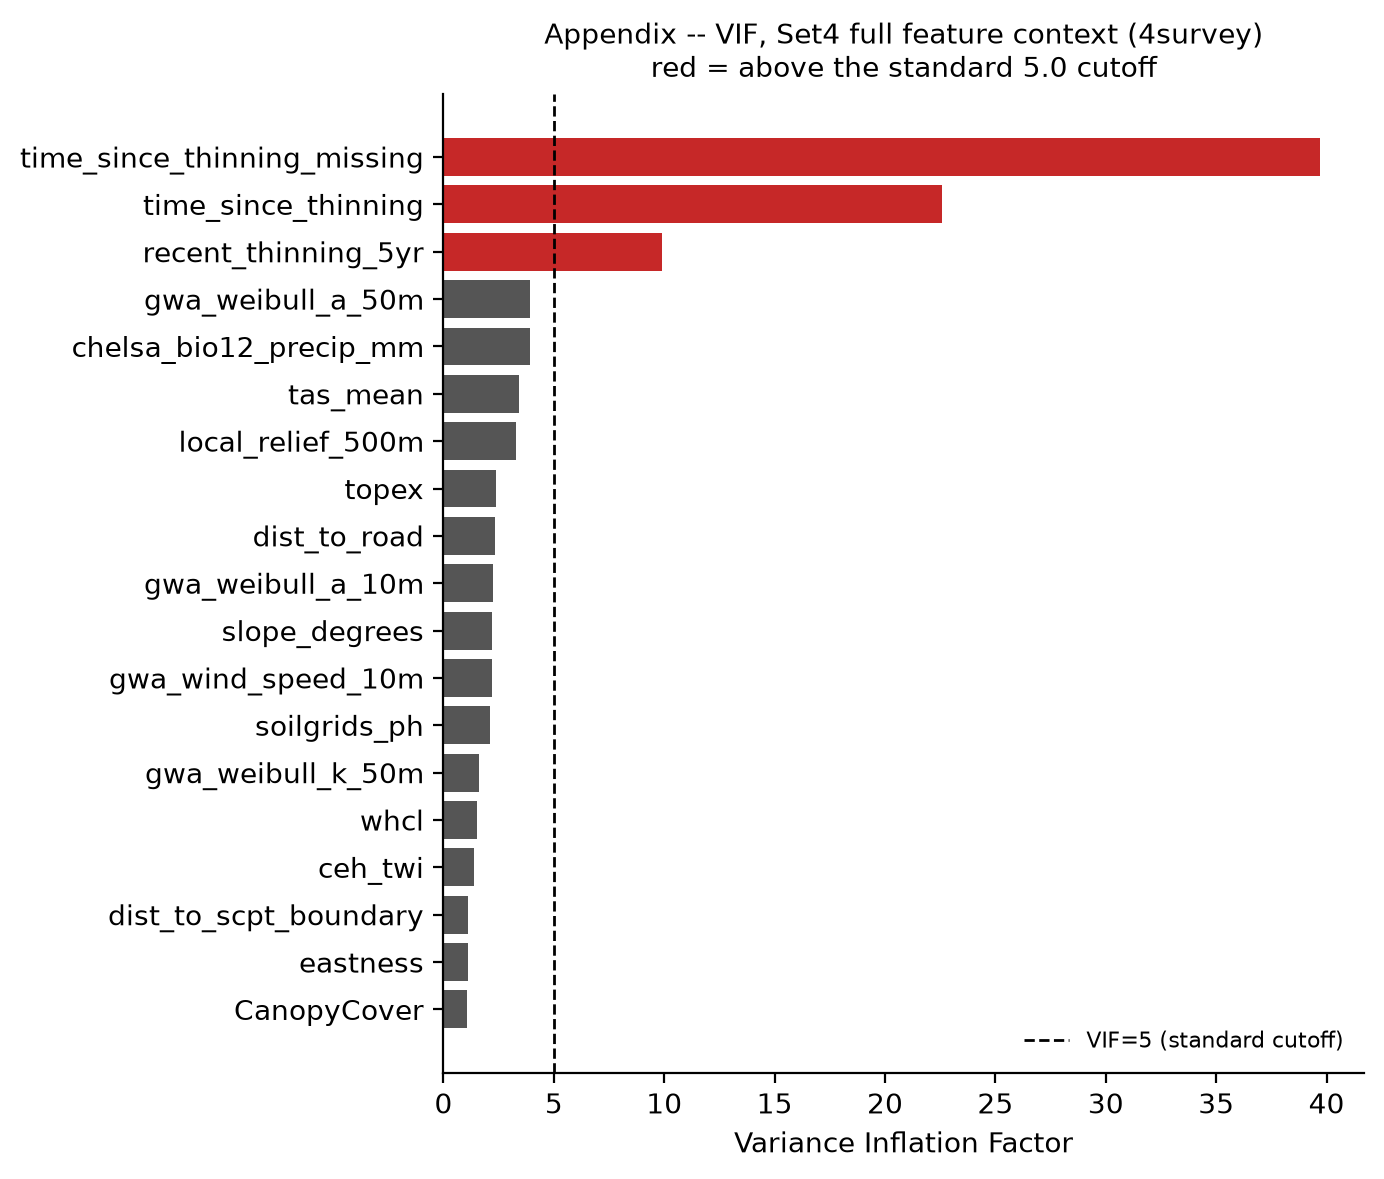
\includegraphics[width=0.6\textwidth]{figures/fig_results/q1/q1_final_appendix_vif.png}
\caption{\small{Variance inflation factor (VIF) for all 19 Set4 columns (4-survey), computed live via \texttt{compute\_vif\_table()}. Only the 3 thinning/management columns exceed the standard VIF=5 cutoff (expected -- \texttt{time\_since\_thinning} and its missingness flag are closely related by construction); all abiotic (terrain/climate/soil) variables discussed in the main text, including the 6 unstable ones, have VIF well under 5, ruling out multicollinearity as their cause.}}
\label{fig:q1-appendix-vif}
\end{figure}

\subsection{Category-level ablation (soil / climate / terrain)}
\label{app:category-ablation}
% AUDIT: placeholder -- referenced once from results_q1 ("full ablation in Appendix~\ref{app:category-ablation}"),
% not yet built here. The headline numbers already quoted in the main text (soil +0.022 R2, climate -0.056 R2,
% Set4 category refit) need their source table/run reproduced and placed here -- not yet done this session.

\section{Q2 appendix}
\label{app:results-q2}

\subsection{Terrain/climate variable reliability, Q1 vs.\ Q2}
\label{app:results-q2-reliability}
% Referenced from results_q2_22_08_0214.tex (the "same terrain variables behave the same
% way" cross-check paragraph). Built 2026-08-23.

\begin{table}[!htbp]
\centering
\scriptsize
\renewcommand{\arraystretch}{1.2}
\begin{tabular}{lp{3.3cm}p{4.2cm}cp{2.8cm}}
\toprule
Variable & Q1: EN vs.\ LMM & Q1 mechanism (if disputed) & Q2: \% cpmt.\ same sign & Read \\
\midrule
CanopyCover & Agree (EN 1.94, LMM 1.86) & not disputed & 100.0 & Reliable everywhere \\
slope\_degrees & Agree (EN 0.99, LMM 0.86) & not disputed & 97.0 & Reliable everywhere \\
chelsa\_bio12\_precip\_mm & Agree (EN $-0.62$, LMM $-1.42$) & not disputed & 87.4 & Reliable everywhere \\
topex & Disagree (EN 0.06, LMM 1.32) & Real local signal (within-cpmt.\ corr.\ 0.214 $>$ raw 0.080) & 71.9 & Real effect, hard for a straight line (global or local) to pin down consistently \\
windward\_topex & not tested in Q1 & n/a & 91.8 & Q2-only variable, more stable than plain topex \\
tas\_mean & Disagree (EN $-0.33$, LMM 0.02) & Artifact (within-cpmt.\ corr.\ 0.090 $\ll$ raw 0.279) & 78.4 & Q1: fake signal, despite a fairly stable local sign in Q2 -- stability alone does not make it a real effect \\
soilgrids\_ph & Disagree (EN 0.12, LMM 0.07) & Artifact (within-cpmt.\ corr.\ 0.035 $\ll$ raw 0.224) & 51.1 & Both chapters agree: not a real effect \\
dist\_to\_road & not tested in Q1 & n/a & 74.9 & No Q1 comparison; moderately stable sign in Q2 \\
\bottomrule
\end{tabular}
\caption{\small{Terrain/climate variable reliability, cross-referenced between Q1 (does a
global Elastic Net model agree with a linear mixed-effects model on a variable's
coefficient, Set4, 4-survey) and Q2 (does GNNWR's own local coefficient keep the same sign
across compartments, Set4, 4-survey, pooled 5 folds, $n=231$ compartments). These are two
genuinely different tests that happen to agree on topex and slope\_degrees -- not the same
measurement repeated.}}
\label{tab:results-q2-reliability}
\end{table}
% Source (internal tracking only, not for the caption): Q1 columns live-recomputed from
% outputs/spatial_block_kfold/rq2_attribution_nested_set4_gated_all_vif/4survey/fold_{0-4}/
% (elastic_net_coefficients.csv, nlme_fixed_effects.json); Q2 column live-recomputed from
% GNNWR's own saved per-plot coef_* columns, same fold files as Table~\ref{tab:results-q2-ablation}.

\subsection{Flagged-plot split diagnostics}
\label{app:flagged-plot-split}
% AUDIT: placeholder -- referenced once from results_q2 (fixed-k curve-fitting artifact vs.\ genuine rapid growth
% in the 266 Tukey-flagged plots). Source diagnostics exist in TEMP_results_attribution/ per earlier session work
% (see handover docs) but have not been transcribed into this appendix yet.

\subsection{Category-level Moran's I diagnostics (with terrain bandwidth-artifact adjustment)}
\label{app:results-q2-category-morans-i}
% AUDIT: placeholder -- results_q2 currently points this content at the generic \ref{chap:appendix} rather than
% a specific label; once this subsection is filled in, update that in-text ref to
% \ref{app:results-q2-category-morans-i} instead.

\section{Q3 appendix}
\label{app:results-q3}

\subsection{Full 6-survey table}
\label{app:results-q3-6survey}
% Moved out of the main Table~\ref{tab:results-q3} 2026-08-23 for clarity, since 6-survey is
% not this chapter's main analysis surface (see that table's caption). PINN/PINN-k rows show
% -- : the corrected-forward-pass work this chapter reports (environment sweep, lambda
% ablation, hyperparameter checks -- see temp_results_pinn/RESULTS_TABLE.md) was all done on
% 4-survey only; 6-survey was never rerun with the corrected architecture, and the pre-fix
% 6-survey numbers are not valid evidence for the corrected model (same reasoning as the
% pre-fix PINN runs excluded from the main table).

\begin{table}[!htbp]
\centering
\scriptsize
\setlength{\tabcolsep}{4pt}
\renewcommand{\arraystretch}{1.2}
\begin{tabular}{lrrr}
\toprule
Model & RMSE${\downarrow}$ & MAE${\downarrow}$ & $R^2{\uparrow}$ \\
\midrule
Linear & $4.877{\pm}0.643$ & $3.619{\pm}0.426$ & $0.509{\pm}0.067$ \\
RF & $4.062{\pm}0.249$ & $3.010{\pm}0.185$ & $0.656{\pm}0.046$ \\
XGBoost (tuned) & $\mathbf{3.656{\pm}0.232}$ & $\mathbf{2.669{\pm}0.183}$ & $\mathbf{0.722{\pm}0.031}$ \\
DNN & $3.903{\pm}0.316$ & $2.867{\pm}0.275$ & $0.684{\pm}0.031$ \\
PINN & -- & -- & -- \\
PINN-$k$ & -- & -- & -- \\
\bottomrule
\end{tabular}
\caption{\small{Model comparison for top-height prediction, 6-survey, Set3,
spatial\_block\_kfold, per-fold mean $\pm$ SD across five folds. n=82{,}614 row-years
(13{,}769 plots). Referenced from the main text's DNN-vs.-XGBoost fold-count and
compartment-subsampling discussion. PINN/PINN-$k$ were not rerun with the corrected
forward pass on this cohort (--); see main-text Table~\ref{tab:results-q3}'s caption.}}
\label{tab:results-q3-6survey}
\end{table}

\subsection{Q3 results tables}
\label{app:results-q3-tables}
% Moved out of the main text 2026-08-24 -- main Q3 results section is capped at 3 tables
% (Table~\ref{tab:results-q3}, Table~\ref{tab:pinn-conditions}, Table~\ref{tab:plausibility-comparison}
% stay in main text). These six are supporting/diagnostic detail, referenced from the main-text
% discussion via \ref{} as normal -- moving them here does not change any in-text reference.

% --- Table: compartment 1129 cross-fold check (unchanged) ---
\begin{table}[!htbp]
\centering
\scriptsize
\begin{tabular}{lrrr}
\toprule
Fold & Split membership & Mean $y_{max}$ deviation & Rows $>$70\,m (of 1484) \\
\midrule
0 & 100\% test & $+12.1$\,m & 72 \\
1 & 95\% train & $+11.5$\,m & 44 \\
2 & 98\% train & $+10.7$\,m & 0 \\
3 & 100\% train & $+15.6$\,m & 0 \\
4 & 100\% validation & $+12.4$\,m & 0 \\
\bottomrule
\end{tabular}
\caption{\small{Compartment 1129's mean $y_{max}$ deviation in each of the 5 spatial-block
folds, by how much of the compartment's own data that fold trained on. Inflation persists (and
does not shrink) even when the model trains on the compartment's own real data.}}
% source: RESULTS_TABLE.md #10
\label{tab:compartment1129-crossfold}
\end{table}

% --- Table: trunk-residual comparison, plain PINN vs. PINN-k ---
\begin{table}[!htbp]
\centering
\scriptsize
\begin{tabular}{lrrr}
\toprule
Fold & Plain PINN trunk mean$|\cdot|$ & PINN-$k$ trunk mean$|\cdot|$ & Ratio \\
\midrule
0 & 0.207 & 0.410 & 1.98$\times$ \\
1 & 0.238 & 0.553 & 2.33$\times$ \\
2 & 0.255 & 0.844 & 3.31$\times$ \\
3 & 0.339 & 0.668 & 1.97$\times$ \\
4 & 0.268 & 0.704 & 2.63$\times$ \\
\bottomrule
\end{tabular}
\caption{\small{Mean absolute size of the shared correction network's output, plain PINN vs.\
PINN-$k$, all 5 folds. PINN-$k$'s correction is larger than plain PINN's in every fold --
roughly $2\times$ or more throughout, not a strict trend.}}
% source: RESULTS_TABLE.md #7. UPDATED 2026-08-24: added fold 3 (ratio 1.97x), completing all
% 5 folds. Fold 3 is just under 2x (1.968), so "consistently above 2x" softened to "roughly 2x
% or more" -- range across all 5 folds is 1.97x-3.31x, no fold below ~1.97x. Earlier "grows
% fold to fold" framing already dropped when fold 4 was added (1.98 -> 2.33 -> 3.31 looked
% monotonic on 3 folds; fold 4 at 2.63 broke it) -- fold 3 confirms this further: not a trend,
% just consistently >=~2x across all 5 folds. All 5 folds now done, nothing pending.
\label{tab:trunk-residual}
\end{table}

% --- Table: error by age band and height band (unchanged) ---
\begin{table}[!htbp]
\centering
\small
\begin{tabular}{lrrrr}
\toprule
Age band (years) & $n$ & DNN MAE & PINN MAE & PINN-$k$ MAE \\
\midrule
15--30 & 29,837 & 2.49 & 2.52 & 2.53 \\
30--45 & 17,861 & 2.69 & 2.85 & 2.93 \\
45--60 & 7,590 & 4.16 & 4.24 & 4.42 \\
60--75 & 2,034 & 4.63 & 5.23 & 5.15 \\
75--93 & 751 & \textbf{6.83} & 6.40 & 6.81 \\
\midrule
Height band & $n$ & DNN MAE & PINN MAE & PINN-$k$ MAE \\
\midrule
0--10\,m & 12,373 & 2.68 & 3.37 & 3.15 \\
10--20\,m & 29,629 & 2.59 & 2.62 & 2.74 \\
20--30\,m & 13,733 & 3.36 & 2.98 & 3.15 \\
30--47\,m & 2,338 & 5.26 & 5.71 & 5.72 \\
\bottomrule
\end{tabular}
\caption{\small{Mean absolute error by tree age and by tree height, DNN vs.\ plain PINN vs.\
PINN-$k$, pooled across all 5 folds (58,073 plots for all three models). Bold: DNN is the
WORST of the three at the oldest ages, not the best -- see note below on how this reverses the
fold-0-only reading.}} % source: RESULTS_TABLE.md #12, updated 2026-08-24, pooled 5-fold
\label{tab:age-height-error}
\end{table}

% --- Table (NEW): selection rule + the two flagship examples ---
% Rule (2026-08-23, replaces earlier ad-hoc picks): among compartments with >=50 pooled
% held-out plots (excludes small-n compartments where 1-2 plots could drive the mean), rank by
% mean deviation for the "systematic site signal" story, and separately by single-plot max/min
% deviation for the "one implausible plot" story. A compartment can lead on one ranking and not
% the other -- that is expected, not a problem, since the two rankings answer different
% questions.
\begin{table}[!htbp]
\centering
\small
\begin{tabular}{llrrl}
\toprule
Compartment & Direction & Mean dev. (m) & Most extreme plot (m) & Why flagged \\
\midrule
1129 & Over & +12.2 (rank 10/178) & \textbf{+25.8 (rank 1/178)} & Single most extreme plot \\
2021 & Under & \textbf{-21.4 (rank 1/178)} & \textbf{-30.4 (rank 1/178)} & Largest mean \emph{and} most extreme plot \\
\bottomrule
\end{tabular}
\caption{\small{The two flagship compartments, ranked among the 178 compartments with
$n\geq50$ pooled held-out plots. 1129 wins on single-plot extremity alone; 2021 wins on both
mean and single-plot extremity.}}
% source: RESULTS_TABLE.md #13, n>=50 reliability rule applied to the pooled 5-fold compartment
% deviation table (58,073 plots).
\label{tab:productivity-flagships}
\end{table}

% --- Table (NEW): the wider top-5-per-side picture, reported honestly (not filtered to
% only the yield-class-confirming rows) ---
\begin{table}[!htbp]
\centering
\small
\begin{tabular}{lrrrlr}
\toprule
Compartment & Mean dev. (m) & $n$ plots & Yield class & Agrees? & Mean age (yr) \\
\midrule
\multicolumn{6}{l}{\textit{Over-productive, top 5 by mean deviation (n$\geq$50)}} \\
2057 & +15.6 & 112 & 10--16 (mixed) & No & 59.8 \\
1130 & +14.6 & 78 & 22--24 & Yes & 33.6 \\
2130 & +14.6 & 98 & 20--24 & Yes & 35.1 \\
1122 & +13.4 & 51 & 24 & Yes & 25.0 \\
1027 & +13.4 & 56 & 12 & No & 72.0 \\
\midrule
\multicolumn{6}{l}{\textit{Under-productive, top 5 by mean deviation (n$\geq$50)}} \\
2021 & -21.4 & 403 & 12 & Yes & -- \\
1070 & -18.1 & 222 & 12 & Yes & -- \\
2094 & -17.7 & 279 & 10--12 & Yes & -- \\
1069 & -11.8 & 297 & 12 & Yes & -- \\
2022 & -10.3 & 417 & 16 & Weakly & -- \\
\bottomrule
\end{tabular}
\caption{\small{Top 5 over- and under-productive compartments by mean deviation
($n\geq50$), checked against independent yield class. Reported as-is, not filtered down to the
rows that agree. Under-productive side agrees with independent yield class in 4/5 cases;
over-productive side agrees in only 3/5, including a disagreement from the single biggest
over-productive signal (2057). The two disagreeing over-productive rows (2057, 1027) are both
old and wind-exposed (mean age 59.8/72.0yr, windward index +15.2/+11.0); the three agreeing
rows (1130, 2130, 1122) are both young and sheltered-to-neutral (mean age 25.0--35.1yr,
windward index -9.5 to +0.4) -- see main-text discussion of this split.}}
% source: RESULTS_TABLE.md #13.
\label{tab:productivity-top5}
\end{table}

% --- Table (NEW): correlation with independent yield-class records ---
\begin{table}[!htbp]
\centering
\small
\begin{tabular}{lrr}
\toprule
Comparison & Pearson $r$ & $n$ \\
\midrule
Plain PINN $y_{max}$ deviation vs.\ yield class & 0.273 & 58,073 \\
PINN-$k$'s $k$ vs.\ yield class & 0.286 & 58,073 \\
PINN-$k$'s $y_{max}$ vs.\ yield class & 0.135 & 58,073 \\
\bottomrule
\end{tabular}
\caption{\small{Correlation between each model's personalisation and the Forestry Commission's
independent yield-class rating -- never a model input, checked against both feature lists.
Pooled across all 5 folds.}}
% UPDATED 2026-08-24: was fold-0-only (n=11,508, PINN-k y_max r=0.334 -- the apparent
% strongest of the three). Pooled data flips the ranking: PINN-k's y_max is now the WEAKEST
% (0.135), its k the strongest (0.286). See RESULTS_TABLE.md section 13 addendum.
\label{tab:yieldclass-correlation}
\end{table}

\subsection{Q3 supporting figures}
\label{app:results-q3-figures}
% Moved out of the main text 2026-08-24 -- same reasoning as Section~\ref{app:results-q3-tables}:
% main Q3 Discussion keeps only the two headline compartment maps (fig:ymax-deviation-map,
% fig:ymax-k-deviation-maps) in the flow; these three are reference/ranking detail one step
% removed from the two flagship examples, not themselves the headline claim. Referenced from the
% main text via \ref{} as normal -- moving them here does not change any in-text reference.

\begin{figure}[!htbp]
\centering
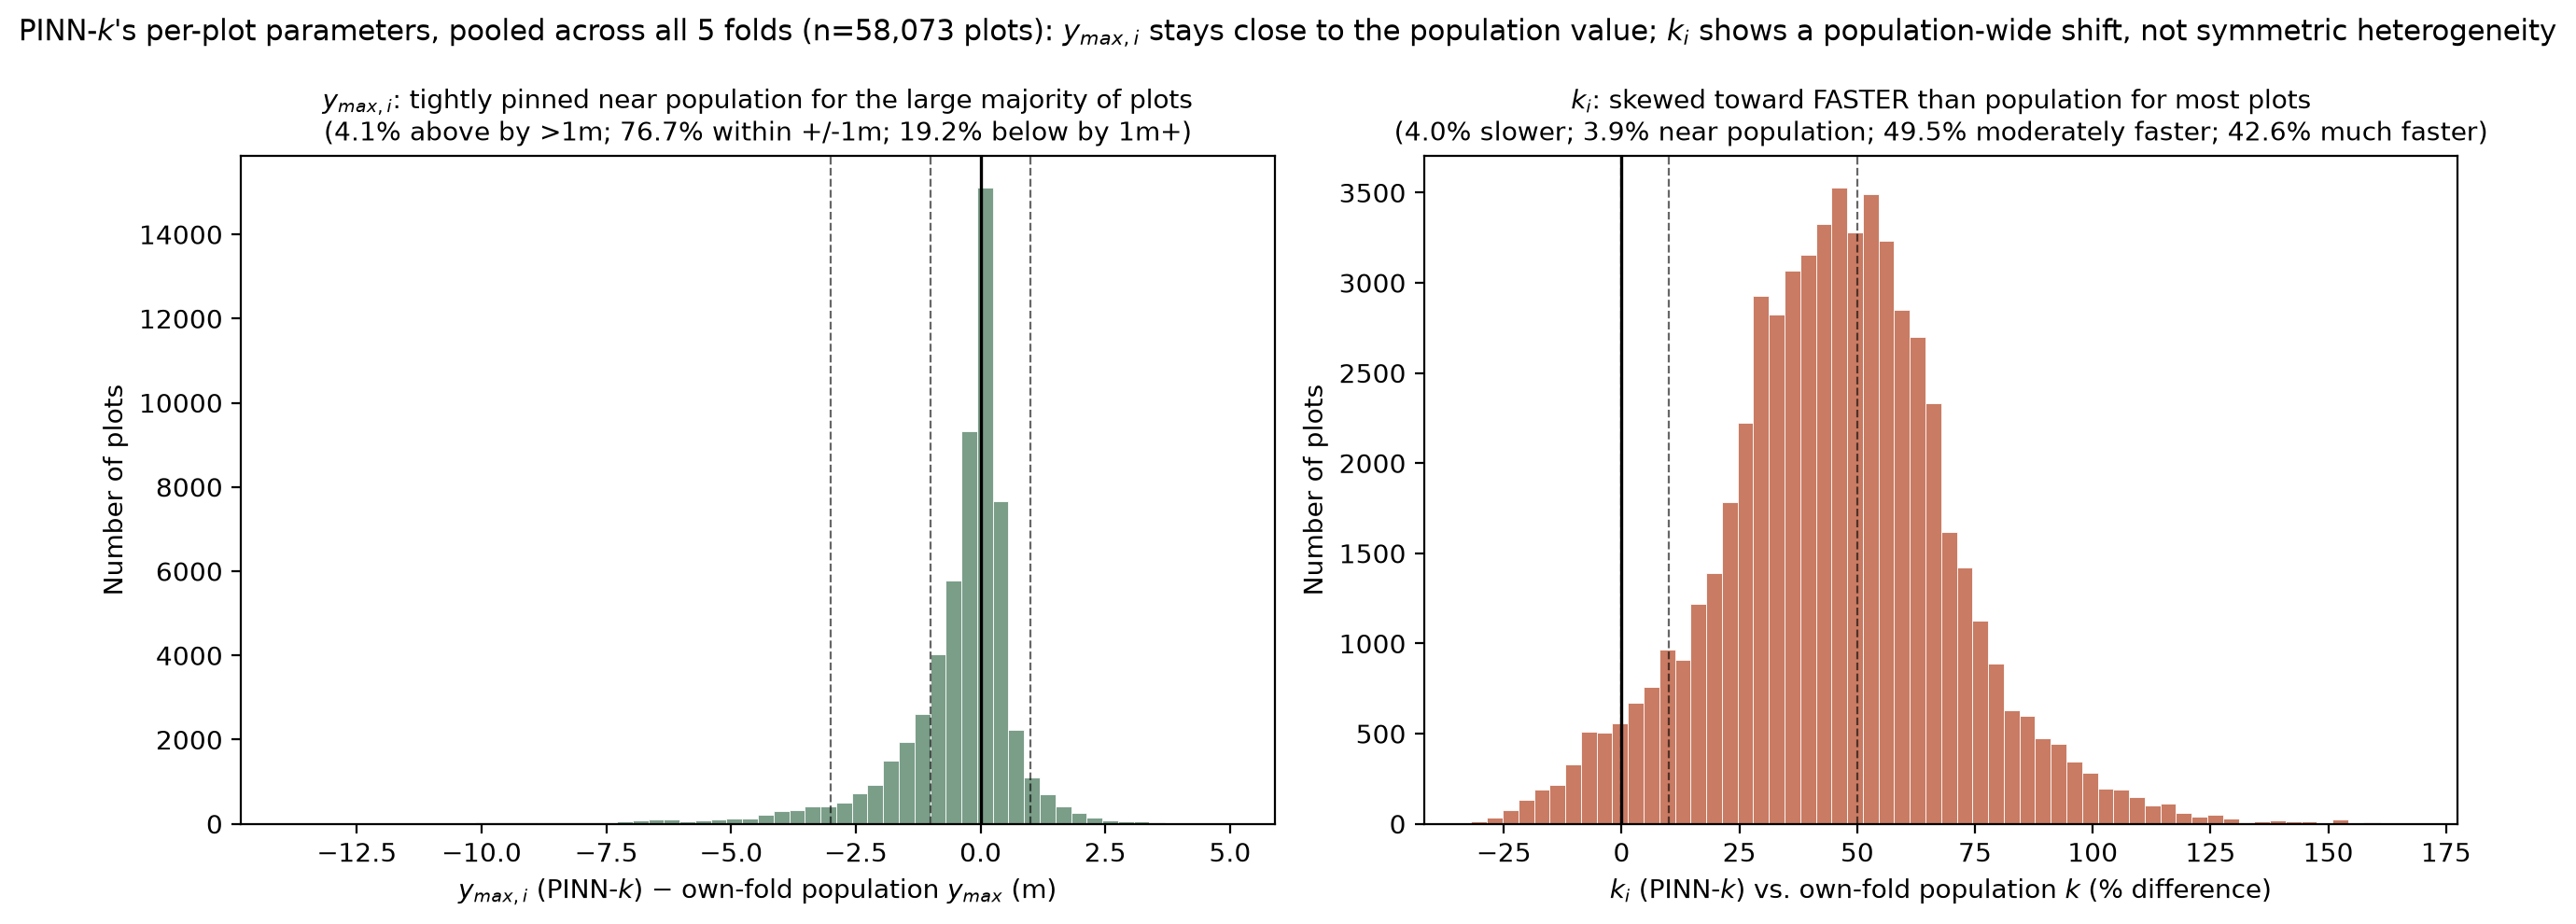
\includegraphics[width=0.95\textwidth]{figures/fig_results/q3/q3_pinn_param_distribution.png}
\caption{\small{PINN-$k$'s per-plot parameters, pooled across all 5 folds (58,073 plots), each
plot's deviation measured against its own fold's population baseline. Left: $y_{max,i}$ stays
tightly pinned near the population value for the large majority of plots (76.7\% within
$\pm$1m). Right: $k_i$ is skewed strongly toward faster than population for most plots (92.1\%
moderately or much faster) -- a population-wide shift, not a symmetric spread of real
heterogeneity. Quantitative companion to Figure~\ref{fig:ymax-k-scatter}'s shape: the same
one-sided $k$ routing, shown as a distribution rather than a scatter.}}
% UPDATED 2026-08-24: pooled across all 5 folds (was fold-0-only, n=11,508) -- same fold-own-
% baseline pooling as load_pooled_pinn_k_deviation_data() in build_q3_redraft_figures.py, to
% avoid the same Simpson's-paradox-style confound already found and fixed in the y_max-vs-k
% scatter figure. Moved into figures/fig_results/q3/ at the same time (was in the flat
% fig_results/ root, unreferenced anywhere). Script:
% models/growth_curve_attribution/q3_pinn_param_distribution_check.py.
\label{fig:pinn-param-distribution}
\end{figure}

\begin{figure}[!htbp]
\centering
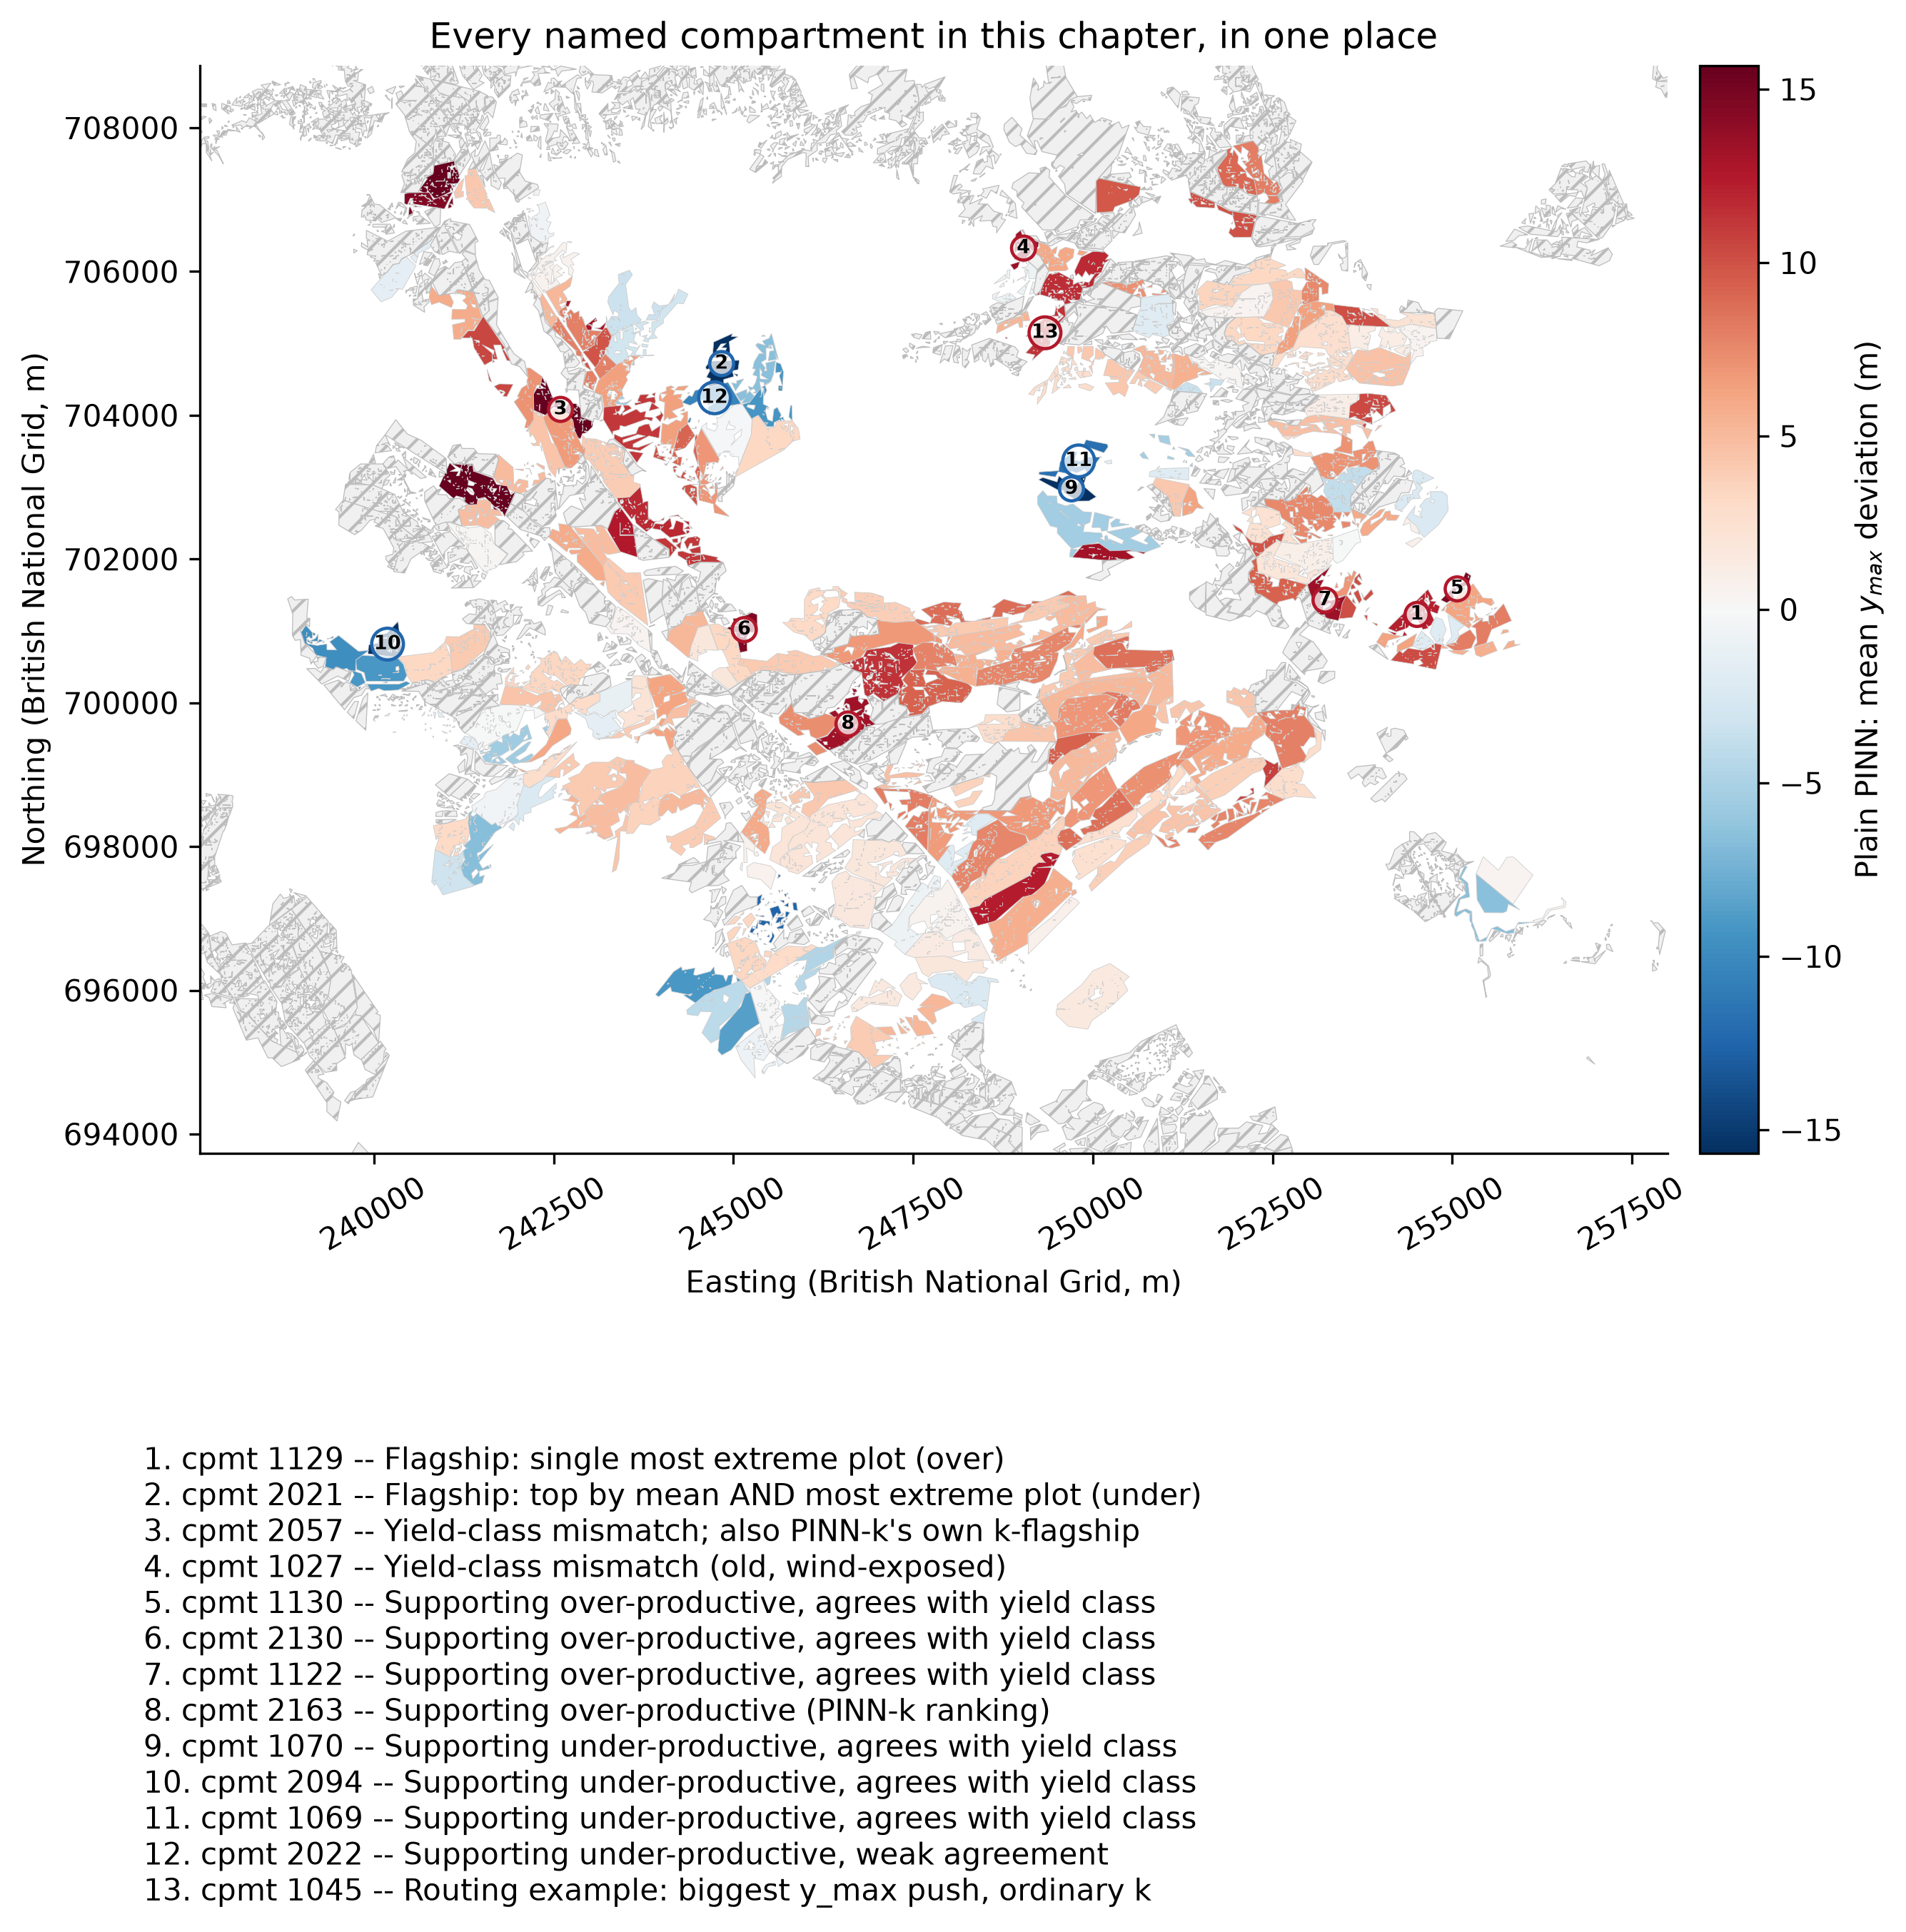
\includegraphics[width=0.95\textwidth]{figures/fig_results/q3/q3_all_compartments_reference_map.png}
\caption{\small{Every compartment named anywhere in this chapter, numbered on one map, with
the reason each was highlighted. A single lookup source -- some compartments here appear in a
table but no other figure, or a figure but no table.}}
% BUILT 2026-08-24. Reference/lookup figure, not tied to one specific paragraph.
\label{fig:all-compartments-reference}
\end{figure}

\begin{figure}[!htbp]
\centering
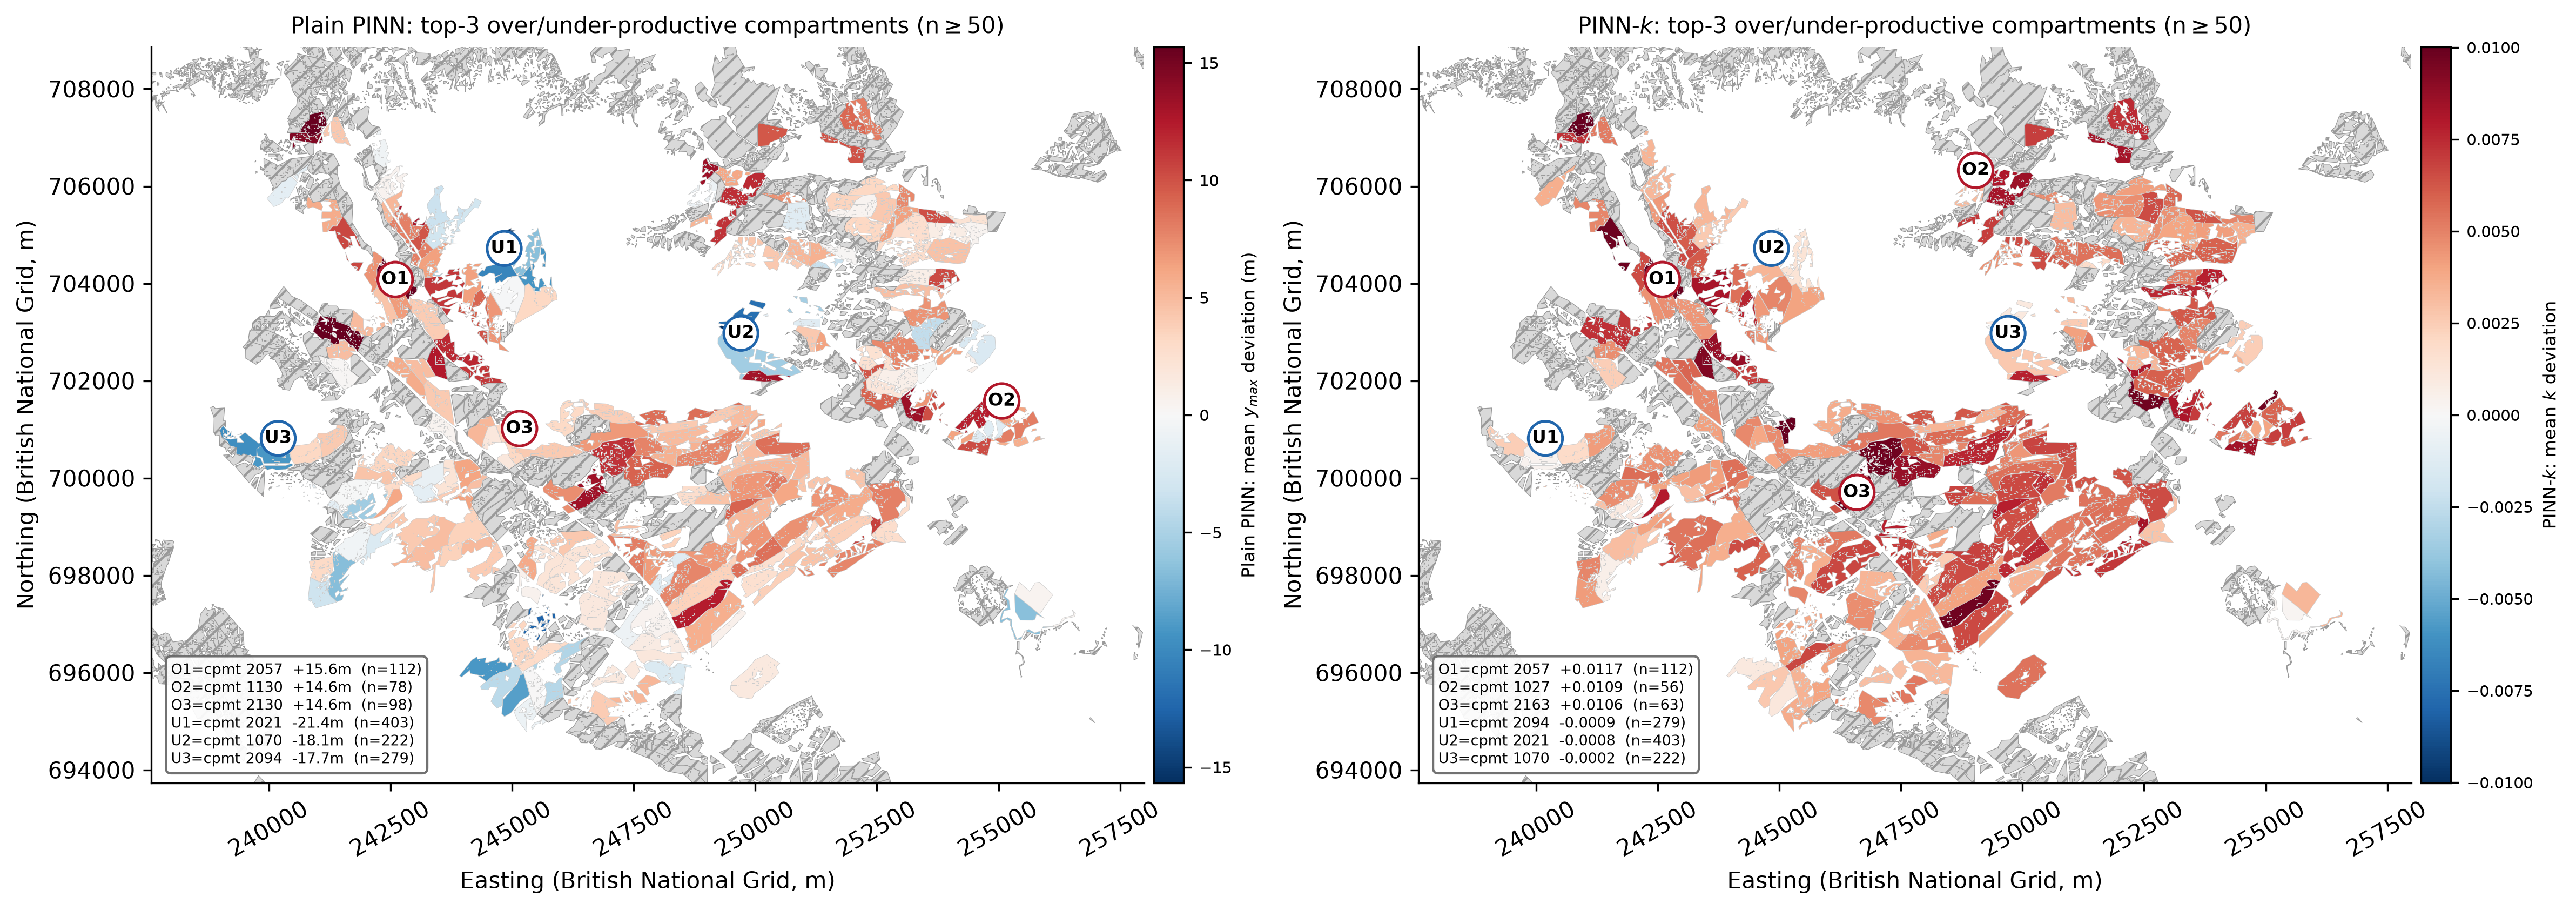
\includegraphics[width=0.95\textwidth]{figures/fig_results/q3/q3_pinn_ymax_hotspot_summary.png}
\caption{\small{Top-3 over- and under-productive compartments (n$\geq$50), plain PINN (left)
vs.\ PINN-$k$ (right). 2057 tops both; the under-productive top-3 is the same three compartments
on both sides, just reordered.}}
\label{fig:hotspot-summary}
\end{figure}

\begin{figure}[!htbp]
\centering
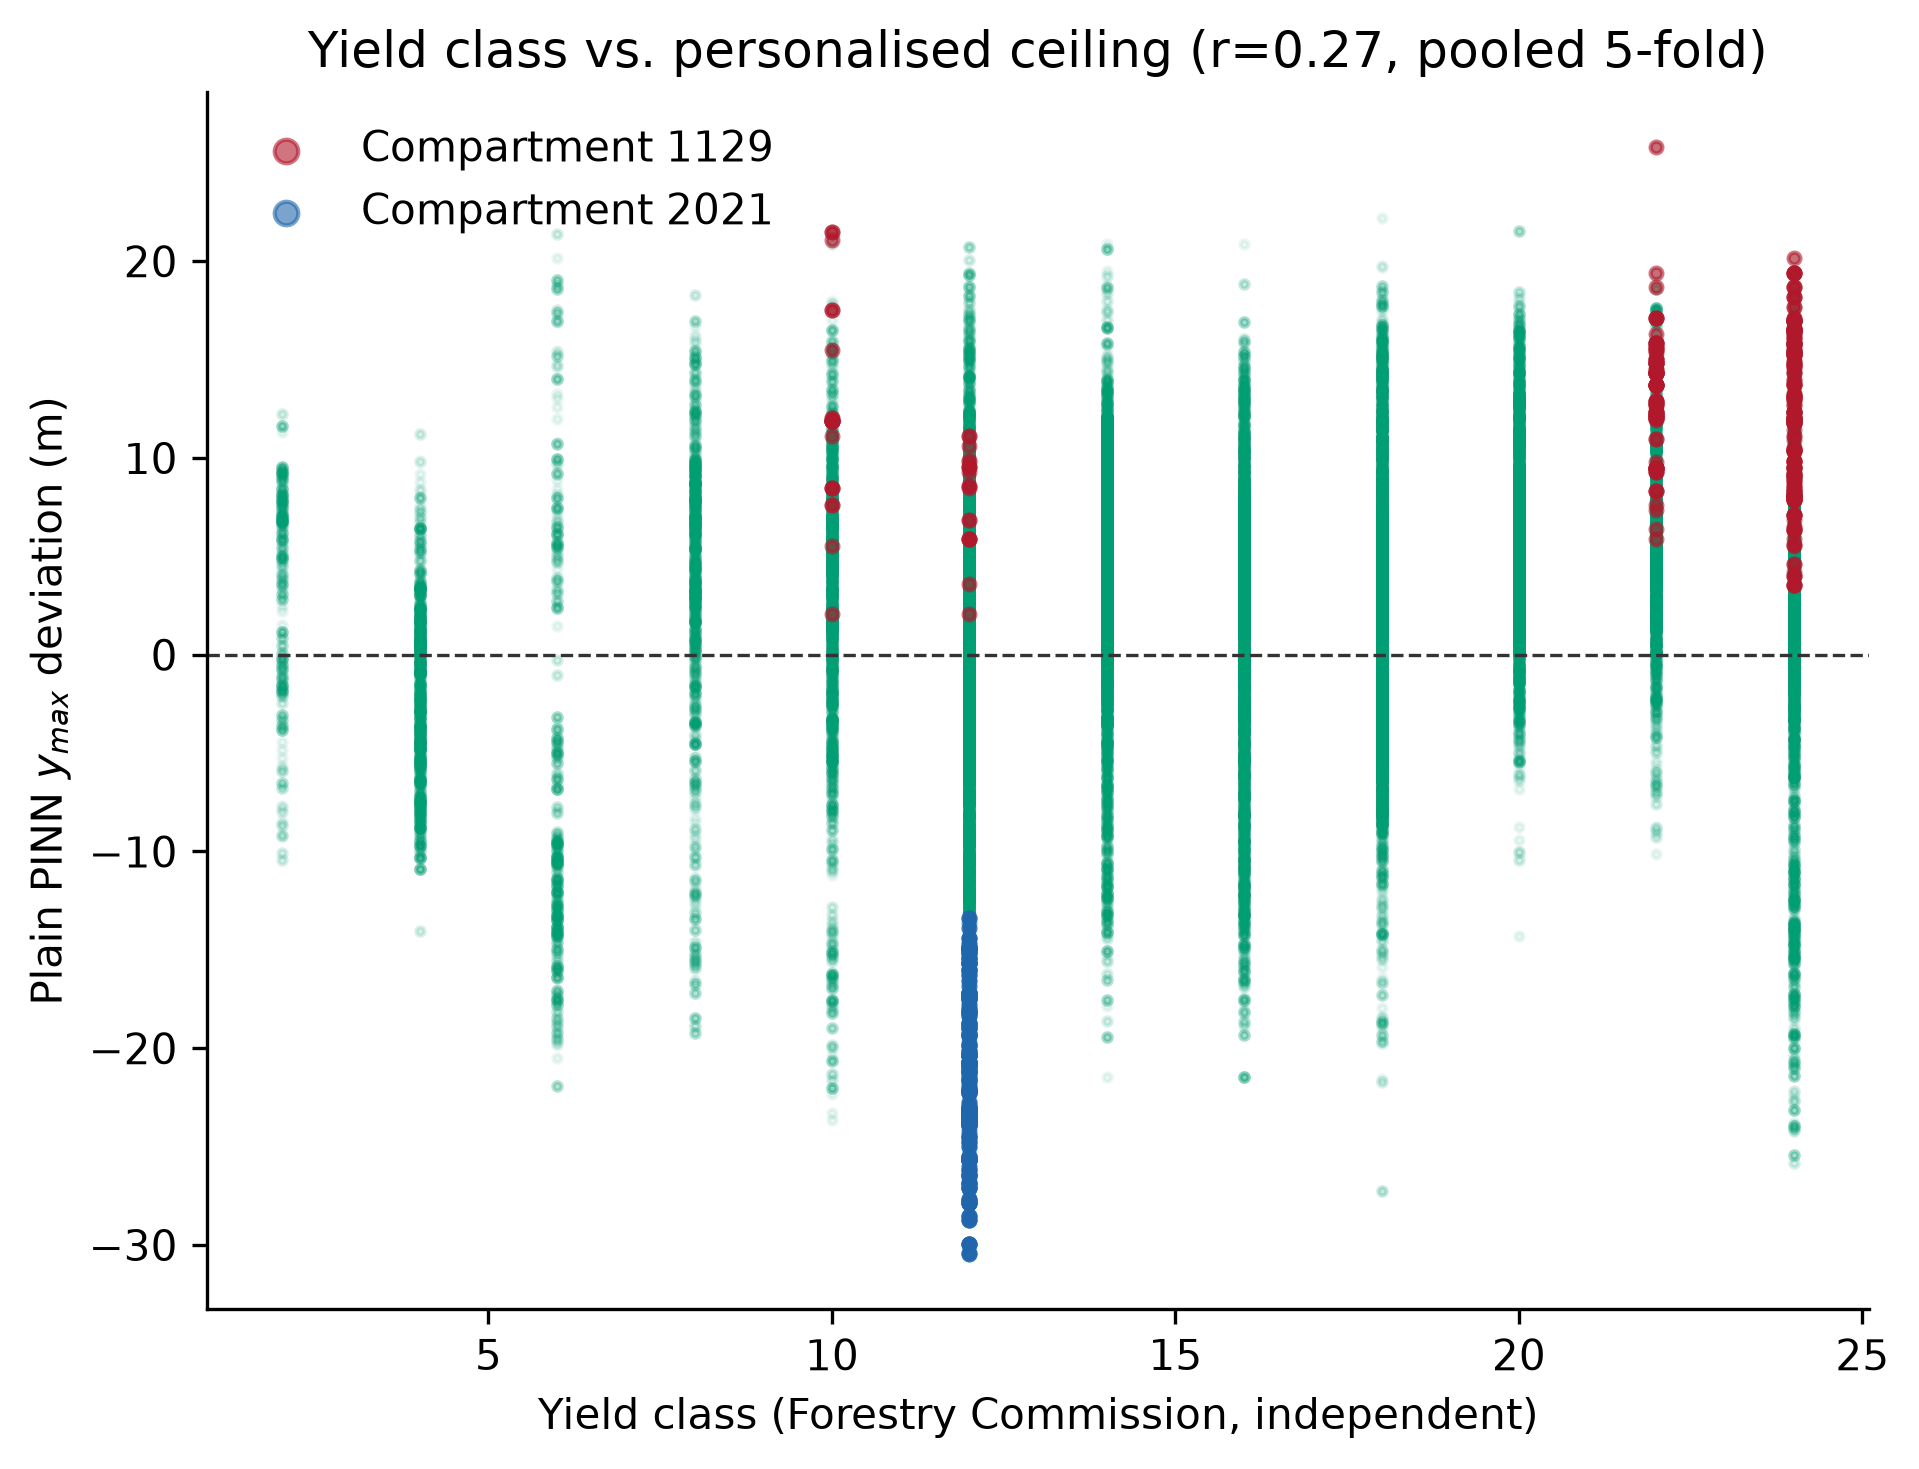
\includegraphics[width=0.7\textwidth]{figures/fig_results/q3/q3_yieldclass_scatter.png}
\caption{\small{Plain PINN's $y_{max}$ deviation vs.\ independent yield class, pooled across
all 5 folds. Green: every held-out test plot (58,073), one dot each -- yield class only takes
about a dozen discrete values, which is why the dots stack into vertical bands rather than
spreading evenly across the x-axis. Red and blue: the same kind of point, restricted to the two
flagship compartments (1129, 2021), so their position within the wider pattern is visible --
1129 clustered high (mostly yield class 22-24), 2021 clustered low and tightly (entirely yield
class 12, strongly negative). The dashed black line is a zero-deviation reference, not a data
series. Real but modest correlation (Table~\ref{tab:yieldclass-correlation}) -- the upward
drift of the whole cloud left to right is what that correlation number is measuring.}}
% REBUILT 2026-08-24 on pooled data (was fold-0-only, n=11,508). Pooling changed the answer
% here more than expected -- see RESULTS_TABLE.md and the note on fig:ymax-k-scatter's build
% comment for why pooling is the correct choice for THIS comparison (yield class has no
% fold-varying baseline to confound, unlike the y_max-vs-k comparison). Source: chat 2026-08-24.
\label{fig:yieldclass-scatter}
\end{figure}

\subsection{Why the broadest feature list looked worse}
\label{app:results-q3-set4}
% Moved out of the main Discussion 2026-08-24 -- secondary caveat, not a headline. Was its own
% \paragraph* in the working file, titled "Appendix: why the broadest feature list looked worse
% -- and why that is a weak finding, not a strong one."
Why the broadest environment list (Set4) seemed to underperform the medium list (Set3): its
extra features are not ignored by the model -- they draw more than their fair share of
permutation importance -- they just do not repay that attention in held-out accuracy as well as
the medium list's more curated features. Caveat: the Set3-vs-Set4 gap this explains is itself
within fold-to-fold noise for plain PINN (Table~\ref{tab:pinn-conditions}), and absent entirely
for PINN-$k$ -- a plausible explanation for a small, uncertain effect, not a solid one.

\subsection{Pre-fix PINN runs (uncorrected baseline, for comparison)}
\label{app:results-q3-prefix-pinn}
% AUDIT: placeholder -- results_q3 currently points this content at the generic \ref{chap:appendix} rather than
% a specific label; once this subsection is filled in, update that in-text ref to
% \ref{app:results-q3-prefix-pinn} instead.
